\documentclass[fleqn,10pt,letterpaper]{article}
\usepackage[top=1in,bottom=1in,left=1in,right=1in]{geometry}
\usepackage[T1]{fontenc}
\usepackage[utf8]{inputenc}
\usepackage{times}
\usepackage{amsmath,amssymb}
\usepackage{graphicx}
\usepackage{hyperref}
\usepackage{url}
\usepackage{enumitem}
\usepackage{titlesec}
\usepackage{multicol}
\usepackage{fancyhdr}
\usepackage{caption}

% -------------------------------------------------------------------------
% Conference heading rules: all-caps primary sections and bold-italic
% subheadings to match the manuscript template.
% -------------------------------------------------------------------------
\titleformat{\section}{\small\bfseries\MakeUppercase}{\thesection}{1em}{}
\titleformat{\subsection}{\small\bfseries\itshape}{\thesubsection}{1em}{}
\titlespacing*{\section}{0pt}{6pt}{4pt}
\titlespacing*{\subsection}{0pt}{5pt}{3pt}

% -------------------------------------------------------------------------
% Footer layout mirrors the conference template.
% Replace the paper ID once the assigned number is available.
% -------------------------------------------------------------------------
\pagestyle{fancy}
\fancyhf{}
\renewcommand{\headrulewidth}{0pt}
\renewcommand{\footrulewidth}{0.4pt}
\lfoot{\small Tangap}
\cfoot{\small \thepage}
\rfoot{\small 40th Annual Small Satellite Conference}

% -------------------------------------------------------------------------
% Keep paragraph and caption styling consistent across the manuscript.
% -------------------------------------------------------------------------
\setlength{\parskip}{3pt}
\setlength{\parindent}{0pt}
\setlength{\mathindent}{0pt}
\captionsetup[table]{font=small,labelfont=bf}
\captionsetup[figure]{font=small,labelfont=bf}

\begin{document}

% -------------------------------------------------------------------------
% Single-column conference front matter.
% -------------------------------------------------------------------------
\begin{flushright}
\textbf{SSC26-X-X}
\end{flushright}

\begin{center}
{\fontsize{12}{14}\selectfont\bfseries Autonomous Satellite Coordination for Planetary Observation: Structural Parity and Bounded-Horizon Non-Convergence\par}
\vspace{0.5cm}
{\small Derick F. Tangap\par}
{\small M.S. Student, Complex Systems Science\par}
{\small Rob Walton College of Global Futures, Arizona State University\par}
{\small Nebula Research Lab\par}
{\small \texttt{dtangap@asu.edu}\par}
\end{center}


\section*{ABSTRACT}

Planetary observation increasingly depends on distributed space systems that can coordinate sensing across large spatial scales, dynamic targets, and constrained onboard resources. Autonomous satellites may expand coverage and responsiveness for future observational architectures, but their coordination logic must be evaluated reproducibly and interpreted conservatively before stronger operational claims are justified.

This paper reports a methods-and-calibration study of a reproducible satellite-network simulation pipeline that transforms empirical orbital snapshots into a notional interaction graph and executes multiple protocol layers over that graph. The study does not claim validated flight autonomy, remote-sensing performance, or measured RF behavior; edges represent a declared graph-construction rule rather than verified communications links.

Three findings are reported. First, the pipeline provides a reproducible framework for analyzing autonomous satellite coordination in observation-oriented mission contexts. Second, the “Regular” and “Enhanced” pipeline variants produce identical reported structural metrics on the same graph instance, establishing structural parity. Third, the autonomy layer does not converge within the fixed step budget despite high local agreement, yielding a bounded-horizon negative result preserved explicitly in the artifact record.

The main conclusion is that structural stability in a satellite-derived interaction graph does not imply decision-dynamical resolution within a bounded autonomy horizon. For planetary-observation mission concepts, the result supports a calibration agenda for thresholds, horizons, and graph assumptions while maintaining a clear boundary between simulation evidence and operational readiness.

Regular and Enhanced pipelines matched exactly on the reported structural metrics (\texttt{global\_efficiency\_full = 0.0976}, \texttt{modularity\_full = 0.9023}, \texttt{lcc\_fraction\_full = 0.9753}, and \texttt{compression\_ratio = 9.2308}), while the autonomy layer remained non-convergent at \texttt{max\_steps = 200} despite high mean local agreement (\texttt{rho\_mean = 0.9160}).

\vspace{0.5cm}
\textbf{Keywords:} Planetary observation; autonomous satellite coordination; distributed space systems; multi-satellite sensing; k-nearest-neighbor graph; graph-based autonomy; structural parity; bounded-horizon non-convergence; autonomy calibration.

% -------------------------------------------------------------------------
% Two-column body text begins after the abstract block.
% -------------------------------------------------------------------------
\begin{multicols}{2}
\setlength{\columnsep}{0.25in}

\section{INTRODUCTION}

Answering fundamental questions in Earth and planetary science increasingly depends on advances in space technology that can operate across large spatial scales, uncertain environments, and dynamically evolving observational targets. Planetary research now routinely depends on architectures that extend beyond a single spacecraft or a single observation mode: landed assets provide the richest in situ measurements, but orbital and distributed sensing are required to study global phenomena, revisit transient events, and build synoptic views of planetary bodies over space and time. In that sense, the engineering problem of how multiple spacecraft coordinate is not peripheral to planetary inquiry; it is one of the enabling conditions for future observation strategies.

This framing is especially relevant to distributed satellite systems and autonomy-enabled mission concepts. Multi-satellite constellations, virtual instruments, and swarm-like observation architectures promise broader coverage, higher temporal sampling, and greater resilience than monolithic platforms, but those benefits depend on coordination mechanisms that remain interpretable, bounded, and technically defensible under realistic constraints. A distributed sensing architecture is scientifically useful only if its local decision rules, information flow, and collective behavior can be evaluated with sufficient rigor to separate plausible coordination from unverified autonomy claims.

That requirement motivates the broader thesis context of this work: decentralized autonomy at scale should be studied through formal technological-network models in which many locally interacting agents can be evaluated without assuming a central controller. Within that larger research direction, planetary and Earth science provide a compelling application class because orbiters, remote sensors, and future observation swarms must often coordinate under communication delay, incomplete knowledge, and limited onboard resources. Yet an important gap remains between the appeal of graph-based autonomy concepts and the evidentiary standard required to treat them as scientifically informative. Structural connectivity in a modeled network does not, by itself, establish operational communications realism, and local agreement among simulated agents does not, by itself, demonstrate mission-ready collective decision capability.

Contemporary smallsat swarm efforts likewise emphasize flight demonstration as a process of characterizing capability limits and development needs rather than merely claiming success.[1,13,14] In this spirit, the present manuscript treats simulation not as a shortcut to operational validation, but as a controlled and reproducible calibration instrument. It categorically avoids implying that (i) notional edges correspond to measured RF links, (ii) simulated protocol outputs correspond to flight-validated autonomy, or (iii) structural graph metrics imply decision-dynamical success.

A practical analog for this conservative posture is provided by staged flight demonstrations, autonomous constellation-management systems, and automated science-planning workflows, where autonomy is introduced as bounded support for navigation, coordination, or planning rather than as immediate fully independent authority.[1,5,10,13,14] This is the correct mental model for the present study: simulation outputs are evidence about a declared model under explicit assumptions, and negative results such as bounded-horizon non-convergence are empirically useful because they help define calibration boundaries rather than conceal them.

The central manuscript objective is therefore narrow and publishable: document a reproducible satellite-network simulation framework, demonstrate structural invariance under pipeline enhancement, report bounded-horizon autonomy non-convergence without spin, and define a calibration path forward for distributed observational architectures. This paper is not trying to prove that autonomous coordination has been solved, that firmware autonomy improves outcomes in an operational sense, or that a notional graph model is equivalent to a validated flight communications network. Instead, it asks a more disciplined question: can a reproducible satellite-derived graph framework preserve structural analysis while honestly revealing whether collective decision dynamics resolve within a bounded autonomy horizon?

The main contributions are as follows:

\begin{itemize}
\item A reproducible graph-based simulation pipeline grounded in empirical orbital snapshots and explicit artifact logging.
\item A parity result showing that Regular and Enhanced pipelines produce identical structural outputs on the same graph instance.
\item A bounded-horizon autonomy result showing non-convergence despite high local agreement under declared stopping criteria.
\item A calibration-oriented interpretation that supports future threshold, horizon, topology, and observational-mission sensitivity analysis without redesigning the entire structural pipeline.
\end{itemize}
The remainder of the paper is organized as follows. Related literature situates the study within graph coordination, decentralized collective decision-making, remote and distributed observation architectures, and cautious analogies to flight autonomy. Methods define the layered data model, graph construction, pipeline structure, protocol logic, and reproducibility harness. Results report structural parity, autonomy outcome, and compression fidelity directly from run artifacts. Discussion interprets the calibration significance of those outcomes for distributed autonomy and observation-oriented mission design. Industry Implications articulates conservative gating guidance when convergence remains unresolved. The paper closes with conclusions, acknowledgments, and references.


\section{RELATED WORK}


\subsection{Graph Interaction Models and Neighbor-Based Coordination}

Nearest-neighbor interaction models are foundational in coordination theory because they make explicit how local update rules, graph connectivity, and switching structure shape collective behavior.[4,6,7] Graph-theoretic treatments of multiagent networks likewise emphasize that agreement is not a default property of a networked system, but a conditional property that depends on topology, weighting, and update assumptions.[6,7] This literature provides the conceptual bridge between structural graph metrics and multiagent coordination analysis.

That literature is directly relevant to the present paper, but it also marks an important boundary. Classical coordination studies typically analyze convergence properties of declared agent-update systems; they do not by themselves justify interpreting a kNN graph derived from orbital-element features as an operational communications topology. The current study therefore borrows the graph-theoretic language of coordination while remaining explicit that its edges are modeling constructs rather than measured links.


\subsection{Decentralized Collective Decisions and Global Resolution}

Decentralized control and collective-decision studies are equally important because they show that local agreement and global resolution are not interchangeable. In spacecraft swarms and related multiagent systems, model predictive control, cyclic-pursuit formations, and distributed flocking laws explicitly expose tradeoffs among stability, responsiveness, and collective behavior.[2,3,7]

This body of work is especially close to the present paper because the main behavioral result is not structural failure, but bounded-horizon non-convergence despite high average agreement. The literature therefore provides a defensible conceptual frame for the paper's negative result: non-convergence under a fixed criterion is not automatically pathological, but may instead indicate that the chosen horizon, thresholds, or update dynamics place the system in a non-resolving regime.


\subsection{Satellite Swarm Autonomy as Cautious Context}

Work on spacecraft swarms and distributed satellite autonomy provides important motivation, but it must be used carefully. This paper uses flight and operations literature strictly as context, not as validation of the present graph abstraction.

\begin{itemize}
\item The Starling mission is explicitly framed as a technology-development and validation effort for cooperative spacecraft groups, which is useful for situating the current paper's calibration-oriented posture.[1]
\item Stanford's navigation research for distributed space systems shows how autonomous tracking, orbit estimation, and inter-satellite bearing-angle processing can be developed as rigorous enabling layers for future multi-spacecraft missions.[13,14]
\item Operational constellation-management and automated science-planning systems show that the threshold for deployable autonomy is much higher than structural consistency or local agreement metrics alone.[5,10]
\end{itemize}
The shared lesson across these studies is that autonomy in space systems is judged not only by whether a distributed architecture is conceptually attractive, but by whether its decision process can be bounded, verified, and trusted under realistic constraints. That is exactly why the present paper keeps its claim set narrow.


\subsection{Autonomous Observation and Distributed Remote Sensing}

The observation literature adds a second motivation layer that is important for this manuscript. Planetary and Earth observation increasingly rely on architectures that can observe large spatial domains, revisit dynamic targets, and combine measurements across multiple platforms rather than depending on a single spacecraft or a single instrument mode. In that setting, autonomous coordination is scientifically relevant because it may eventually support when, where, and how distributed assets allocate sensing opportunities under limited power, pointing, compute, and communications budgets.[11,12]

Remote-sensing literature likewise emphasizes that scientific return is limited not only by instrument design, but also by coverage constraints, information-content limits, calibration burdens, and data-processing bottlenecks.[11,12] Recent autonomous-observation efforts make the same point operationally: onboard systems are being developed to screen targets, prioritize anomalies, avoid unproductive observations, and respond to transient events, while distributed observation programs increasingly envision heterogeneous networks that cooperate across platforms.[9,15,16,17,18]

Those studies do not validate the present graph abstraction, but they do clarify why the present question matters. If future planetary-observation architectures are to rely on multiple satellites, adaptive sensing, or opportunistic retargeting, then the coordination logic beneath those capabilities must first be shown to be reproducible, bounded, and interpretable. The current paper therefore addresses an enabling layer of autonomous observation rather than claiming direct measurement improvement or payload-level scientific performance.


\subsection{Reproducibility and Audit-Ready Computational Studies}

The final literature strand concerns reproducibility itself. For a simulation-centered autonomy paper, reproducibility matters because a structurally plausible result is not yet a credible scientific result unless the configuration, graph instance, and outputs can be independently inspected and reproduced.

That requirement is not always foregrounded in graph-coordination or swarm-autonomy literature, where methodological novelty can overshadow artifact discipline. The current study differentiates itself by treating auditability as part of the contribution rather than as a post hoc convenience. The paper's novelty is therefore not a claim to stronger autonomy, but a more defensible combination of three things: an explicitly notional satellite-derived graph model, a parity test between regular and enhanced pipelines on the identical graph instance, and honest reporting of bounded-horizon non-convergence within an artifact-governed workflow.


\section{METHODS}


\subsection{Study Design and Scope Boundary}

This study was designed as a computational methods-and-calibration study rather than as a flight-validation experiment. The workflow preserved a three-layer abstraction boundary so that the scientific claim remained narrow and auditable. In application terms, the study did not attempt to model instrument physics, observation quality, or science return directly; instead, it evaluated a coordination substrate that could eventually matter for future autonomous observation architectures.

\noindent\textbf{Layer A -- empirical orbital-element inputs.}
The input layer consisted of publicly distributed orbital-element records stored as JSON catalogs for Iridium Next, OneWeb, and Starlink. These records served as empirical catalog inputs rather than as direct measurements of intersatellite communication behavior. If the source records originated from NORAD GP/TLE-family products, they should be interpreted as mean-element data that are valid only under compatible SGP-family propagation assumptions.[8]

\noindent\textbf{Layer B -- constructed interaction graph.}
The network layer was a declared k-nearest-neighbor (kNN) graph built from orbital-element features. Edges therefore represented a notional coordination topology, not measured crosslinks or validated RF reachability. This distinction was maintained because nearest-neighbor graphs are useful abstractions for local interaction studies, but they do not by themselves establish operational communication realism.[4,6] In the present framing, this graph should be understood as a coordination scaffold that could someday support distributed observation functions such as sensing allocation, measurement synchronization, or bounded retargeting, rather than as a validated representation of any deployed observing system.

\noindent\textbf{Layer C -- simulated protocol outputs.}
The output layer consisted of software-generated diagnostics, autonomy summaries, and compression metrics produced under fixed code, parameters, and stopping rules. The interpretation of these outputs was therefore limited to properties of the declared model and configuration rather than to flight-qualified autonomy claims. Accordingly, the present outputs should be read as calibration evidence about whether a distributed coordination layer resolves under declared assumptions, not as direct evidence of observation quality, target-detection performance, or mission-level science yield.


\subsection{Data Sources, Ingestion, and Provenance}

The reproducibility package currently contained three raw input catalogs labeled \texttt{Iridium Next.json}, \texttt{OneWeb.json}, and \texttt{Starlink.json}, each treated as an empirical orbital catalog snapshot. The data-handling policy required raw files to remain immutable, all transformations to be script-based, processed outputs to be written deterministically, and any data refresh to be recorded with timestamped provenance metadata.

Each graph node corresponded to one unique \texttt{NORAD\_CAT\_ID}. Preserved node attributes included \texttt{OBJECT\_NAME}, \texttt{OBJECT\_ID}, \texttt{EPOCH}, \texttt{MEAN\_MOTION}, \texttt{ECCENTRICITY}, \texttt{INCLINATION}, \texttt{RA\_OF\_ASC\_NODE}, \texttt{ARG\_OF\_PERICENTER}, and \texttt{MEAN\_ANOMALY}. Input validation required non-zero file size, valid JSON parsing, non-empty record count, and presence of required identifier and orbital-element fields.

The present artifact set did not yet record the exact public source URL, retrieval UTC, or license/usage note for each raw catalog file, and these items should be inserted before submission:

\begin{itemize}
\item \url{https://celestrak.org/NORAD/elements/gp.php?GROUP=iridium-NEXT&FORMAT=json}
\item \url{https://celestrak.org/NORAD/elements/gp.php?GROUP=oneweb&FORMAT=json}
\item \url{https://celestrak.org/NORAD/elements/gp.php?GROUP=starlink&FORMAT=json}
\item Exact local retrieval UTC was not preserved in the current artifact set. During provenance review, the CelesTrak source platform page reported ``Current as of 2026 Mar 30 12:22:26 UTC.''
\item CelesTrak redistributes current GP element sets. Final submission should cite CelesTrak as the source platform and verify any additional reuse or attribution language required at the time of submission.
\end{itemize}
The processed node artifact preserved record-level \texttt{EPOCH} values for individual objects rather than documenting a single common propagated epoch. The manuscript should therefore state the exact temporal interpretation used in graph construction:

\begin{itemize}
\item The graph preserved native record-level catalog epochs as provided in the source snapshots; no separately archived common-epoch propagation step is documented in the current artifact bundle.
\item This interpretation is supported by \texttt{graph\_nodes.csv}, which stores one \texttt{epoch} value per node, and by the current graph-building implementation, which copies each record's \texttt{EPOCH} field into node metadata. The resulting graph should therefore be interpreted as a coordination scaffold built from snapshot orbital fields rather than from a uniformly propagated common-epoch state.
\end{itemize}

\subsection{Graph Construction}

The frozen v1 graph rule was a normalized orbital-feature kNN construction. The feature vector was
\texttt{[MEAN\_MOTION, INCLINATION, RA\_OF\_ASC\_NODE, MEAN\_ANOMALY, ECCENTRICITY]}, and Euclidean distance was computed after z-score normalization. Directed kNN links were then symmetrized into an undirected weighted graph with default \texttt{k = 6}. Edge weights were deterministic and defined as \texttt{1 / (1 + distance)}. Records were sorted by \texttt{NORAD\_CAT\_ID} before graph construction, and fixed feature ordering was used to preserve deterministic outputs.

For the evaluation reported here, the processed graph metadata recorded \texttt{node\_count = 3000}, \texttt{edge\_count = 11990}, and graph signature \texttt{379e28fdce5813b977a4ea1ae04873a2f56256b0dd3e13e84cb5d385327ec025}. These metadata should be cited as the canonical graph-specification artifact in the paper.

Several implementation details remain insufficiently documented in the current artifact bundle and should be stated explicitly in the manuscript rather than left implicit:

\begin{itemize}
\item Z-score normalization was applied globally across the merged catalog, not separately by source file.
\item No explicit secondary manuscript-level tie-break rule is implemented beyond the \texttt{cKDTree} neighbor query; during undirected symmetrization, repeated node pairs are resolved by retaining the minimum distance observed for that pair.
\item Records were loaded from all JSON catalogs in sorted filename order, deterministically sorted by \texttt{NORAD\_CAT\_ID}, \texttt{OBJECT\_ID}, and \texttt{OBJECT\_NAME}, deduplicated by \texttt{NORAD\_CAT\_ID} while keeping the first post-sort record, and then truncated to the first 3000 records. No separate constellation-balancing rule was applied.
\item No additional row-drop stage was applied inside \texttt{build\_graph.py}; rows were excluded only if they failed validation, were removed as duplicate \texttt{NORAD\_CAT\_ID} entries during deterministic deduplication, or fell beyond the \texttt{max\_nodes = 3000} cutoff.
\end{itemize}

\subsection{Pipeline Variants: Regular and Enhanced}

The regular and enhanced pipelines were executed on the same reconstructed graph instance in order to isolate the effect of inserting an autonomy layer without changing downstream structural processing. Both variants began with Stage 1 diagnostics. The regular pipeline then proceeded directly to Stage 2 compression and Stage 3 structural measurement. The enhanced pipeline inserted an autonomy protocol between Stage 1 and Stage 2, then ran the same compression and measurement stages used by the regular pipeline.

Stage 1 computed localized graph diagnostics including weighted degree, approximate betweenness centrality, eigenvector centrality, clustering, and edge betweenness. Approximate betweenness used a sampling setting of \texttt{betweenness\_samples = 200} to keep runtime practical on the 3000-node graph. Critical nodes were defined as the top 10\% of nodes ranked by betweenness, and significant edges were defined as the top 5\% by edge betweenness.

This design made the parity question methodologically clean: if the same graph, compression routine, and Stage 3 measurements were used in both branches, then any structural mismatch would indicate pipeline drift rather than a purely conceptual difference between “Regular” and “Enhanced.” For observation-oriented mission concepts, that distinction matters because an autonomy insertion is only useful if it can be studied without silently altering the structural analysis backbone on which later coordination or sensing studies would depend.[5,10]


\subsection{Autonomy Protocol and Stopping Criteria}

The enhanced pipeline executed the autonomy layer after Stage 1 and before graph compression. Edge weights for the autonomy update were derived from Stage 1 localized metrics by preferring betweenness centrality, falling back to weighted degree, and then to plain degree if needed. Each undirected edge was assigned the average centrality of its endpoints, and the resulting adjacency weights were normalized so that the maximum weight was 1.

If no external input vector was supplied, the local input term \texttt{I} was set to zero for all nodes. If no initial state was supplied, each node state was initialized uniformly in \texttt{[-0.1, 0.1]} using fixed random seed \texttt{42}. The protocol then executed synchronous rounds over the full graph. For node \texttt{i}, the continuous update used the prior state, local input, and weighted neighbor coupling through \texttt{tanh(x\_j(t))}:

\begin{equation}
x_i(t+1) = (1-\alpha)x_i(t) + \alpha \left( I_i + \sum_j w_{ij}\tanh(x_j(t)) \right)
\label{eq:autonomy_update}
\end{equation}

After this continuous update, each node computed a local crowd statistic by averaging its updated value with its neighbors' pre-round states and taking the sign of that average as a local discrete vote \texttt{y\_hat}. Local agreement \texttt{rho} was then defined as the fraction of neighbors whose sign matched that local vote, with isolated nodes assigned \texttt{rho = 1.0}. A confidence-like statistic \texttt{q} was defined as the magnitude of the local average.

At the end of each round, the global label history was updated from the sign of the mean post-round state. The implementation mapped positive mean state to decision label \texttt{A}, negative mean state to \texttt{B}, and exact zero to \texttt{A} by tie rule. Convergence was declared only when all four conditions held simultaneously: population variance of the state vector was below \texttt{theta\_var}, the minimum node agreement was at least \texttt{theta\_agree}, at least \texttt{K\_stable} rounds had been recorded, and the last \texttt{K\_stable} global labels were identical. If these conditions were not met by \texttt{max\_steps}, the run terminated with \texttt{converged = False}, \texttt{decision = None}, and \texttt{rounds = max\_steps}.

The logged autonomy configuration for the reported evaluation was \texttt{alpha = 0.1}, \texttt{theta\_var = 0.01}, \texttt{theta\_agree = 0.8}, \texttt{K\_stable = 5}, \texttt{theta\_high = 0.9}, \texttt{theta\_low = 0.5}, \texttt{use\_synergy\_gate = false}, and \texttt{max\_steps = 200}. Because \texttt{use\_synergy\_gate} was disabled, \texttt{theta\_high} and \texttt{theta\_low} were retained as logged configuration fields but were not active convergence gates in this run.


\subsection{Compression Stage and Structural Metrics}

Stage 2 compression used Louvain community detection with \texttt{random\_state = 42} and preserved critical nodes as singleton super-nodes so that high-betweenness structures remained visible after coarsening. Non-critical nodes were grouped by Louvain community, and edge weights between compressed super-nodes were accumulated by summing contributing inter-group edge weights. Compression ratio was defined as original node count divided by compressed node count.

Stage 3 measured the structural outputs exported for paper assembly. The regular-versus-enhanced comparison reported \texttt{global\_efficiency\_full}, \texttt{avg\_path\_length\_full}, \texttt{modularity\_full}, \texttt{lcc\_fraction\_full}, and \texttt{compression\_ratio}. The autonomy summary reported \texttt{converged}, \texttt{decision}, \texttt{rounds}, \texttt{rho\_mean}, \texttt{rho\_min}, \texttt{rho\_max}, \texttt{q\_mean}, \texttt{x\_mean}, and \texttt{x\_std}. The compression-fidelity export reported \texttt{global\_efficiency}, \texttt{avg\_path\_length}, \texttt{modularity}, \texttt{lcc\_fraction}, and \texttt{compression\_ratio} in full-versus-compressed table form.

Average path length was defined by implementation as finite only for connected graphs and \texttt{inf} otherwise. This rule should be stated explicitly in the manuscript because it determines how disconnected graph instances are represented in the exported results.


\subsection{Reproducibility and Transparency Record}

The evaluation was structured as an artifact-driven reproducibility package. Canonical artifacts included the processed graph specification (\texttt{graph\_metadata.json}), processed node and edge tables (\texttt{graph\_nodes.csv}, \texttt{graph\_edges.csv}), run configuration (\texttt{run\_config.json}), structural comparison table (\texttt{regular\_vs\_enhanced\_metrics.csv}), autonomy summary (\texttt{autonomy\_convergence\_summary.csv}), and compression-fidelity table (\texttt{compression\_fidelity\_table.csv}). The graph metadata artifact recorded the graph signature SHA-256 hash, and the run configuration artifact recorded the autonomy-configuration SHA-256 hash \texttt{330e040ec900889345eea2b714f8d5b345a3f68c5d18c548c159ae17a6c2f1f3}.
The reproducibility package and graphical visual database outputs are distributed through the project repository at \url{https://github.com/nebularesearchlab-commits/NRL-M5-SatSim}, with generated figures stored under \texttt{results/figures/}.

The notebook-based execution record showed the following execution command:

\texttt{python3 "satellite-rerun-ssc26/src/run\_satellite\_rerun.py" --graph-metadata "satellite-rerun-ssc26/data\_processed/graph\_metadata.json" --results-dir "satellite-rerun-ssc26/results" --betweenness-samples 200 --alpha 0.1 --theta-var 0.01 --theta-agree 0.8 --k-stable 5 --max-steps 200}

To satisfy the expectations of a fully reproducible Methods section, the manuscript should still add the missing environment and software details:

\begin{itemize}
\item Python 3.9+
\item The archived rerun does not record exact installed versions. The preserved dependency specification is: \texttt{networkx>=3.0,<4}, \texttt{numpy>=1.20,<3}, \texttt{pandas>=1.3,<3}, and \texttt{python-louvain>=0.16}.
\item No pinned lockfile, environment export, or container reference is currently preserved in the archived artifact bundle.
\item No repository DOI, archival package identifier, or submission archive identifier is currently recorded in the present file set.
\end{itemize}
No human participants, animal subjects, or controlled operational spacecraft were involved in this computational study. The paper's transparency obligation was therefore not human-subject ethics review, but accurate provenance, reproducibility, and conservative claim scope.


\section{RESULTS}


\subsection{Structural Parity}

The regular and enhanced pipelines produced identical reported structural outputs on the same graph instance with graph signature \texttt{379e28fdce5813b977a4ea1ae04873a2f56256b0dd3e13e84cb5d385327ec025}.

\begin{center}
\captionof{table}{Compact evaluation summary for the reported run.}
\label{tab:key_metrics}
\small
\begin{tabular}{lc}
\hline
Metric & Value \\
\hline
global\_efficiency\_full & 0.0976 \\
modularity\_full & 0.9023 \\
lcc\_fraction\_full & 0.9753 \\
compression\_ratio & 9.2308 \\
max\_steps & 200 \\
rho\_mean & 0.9160 \\
converged & False \\
\hline
\end{tabular}
\end{center}


\noindent\textbf{Table 1.} Regular versus Enhanced structural metrics on the identical graph instance.

\begin{table}[t]
\centering
\caption{Regular versus Enhanced structural metrics on the identical graph instance.}
\label{tab:parity_metrics}
\small
\begin{tabular}{lccc}
\hline
Metric & Regular & Enhanced & Match \\
\hline
global\_efficiency\_full & 0.0976056277 & 0.0976056277 & Yes \\
avg\_path\_length\_full & inf & inf & Yes \\
modularity\_full & 0.9022723828 & 0.9022723828 & Yes \\
lcc\_fraction\_full & 0.9753333333 & 0.9753333333 & Yes \\
compression\_ratio & 9.2307692308 & 9.2307692308 & Yes \\
\hline
\end{tabular}
\end{table}

All reported structural metrics matched exactly between the two pipeline variants in the exported comparison table. The logged full-network average path length was \texttt{inf} in both runs. For the paper's observation-oriented framing, this result matters because it shows that inserting the autonomy layer did not distort the downstream structural-analysis backbone. Any later use of this framework for autonomous observation studies would therefore begin from a pipeline whose reported structural outputs remained invariant under the enhanced insertion in this evaluation.

\begin{figure}[t]
\centering
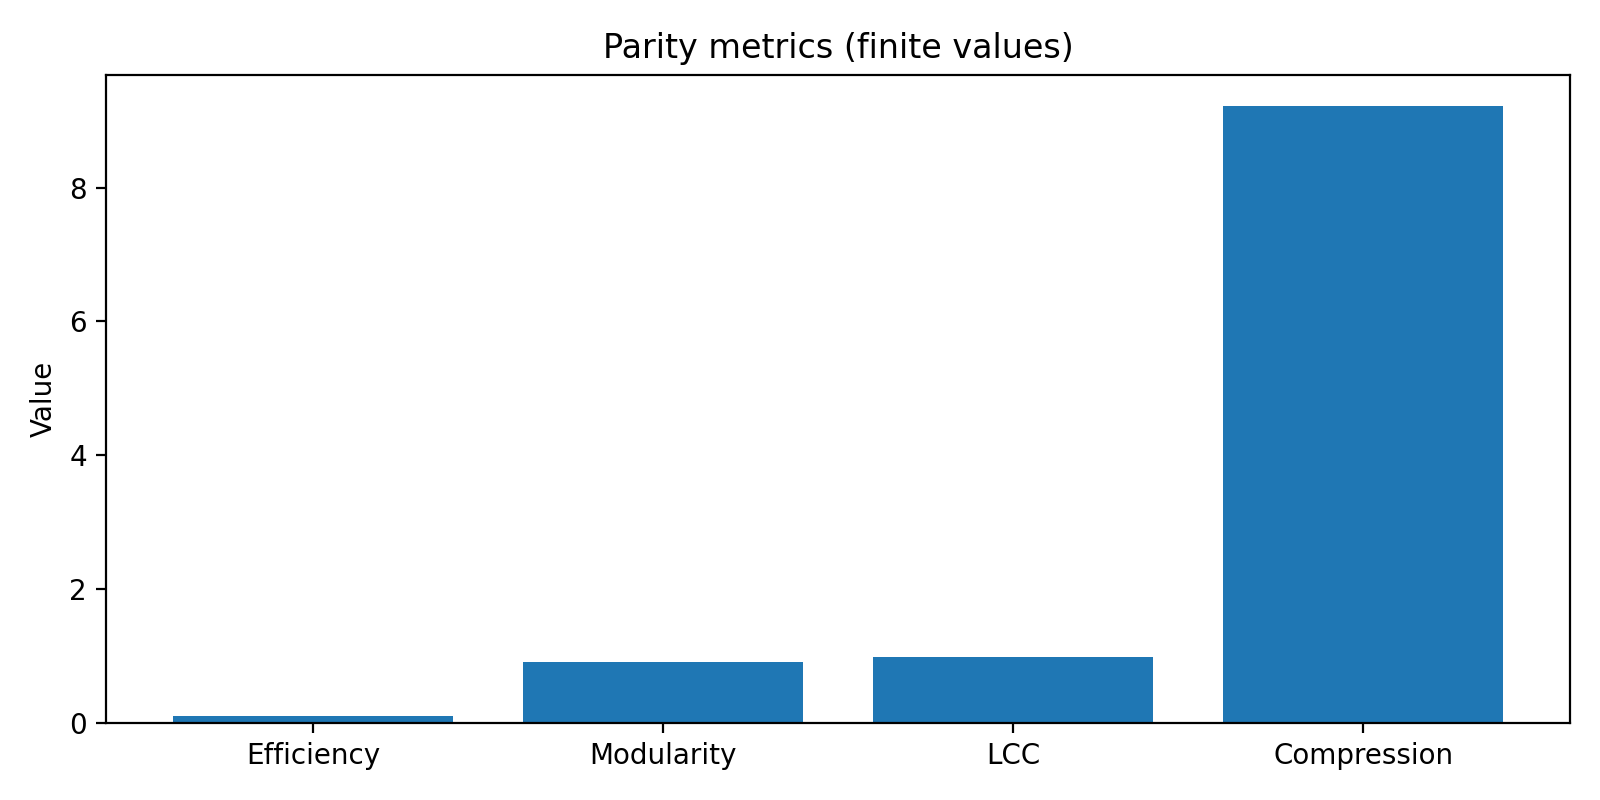
\includegraphics[width=0.92\columnwidth]{../results/figures/fig_parity_metrics.png}
\caption{Parity visualization for the finite reported structural metrics. \texttt{avg\_path\_length\_full} is omitted because both runs reported \texttt{inf}.}
\label{fig:parity_metrics}
\end{figure}


\subsection{Autonomy Bounded-Horizon Outcome}

Under the logged autonomy configuration \texttt{alpha = 0.1}, \texttt{theta\_var = 0.01}, \texttt{theta\_agree = 0.8}, \texttt{K\_stable = 5}, \texttt{theta\_high = 0.9}, \texttt{theta\_low = 0.5}, \texttt{use\_synergy\_gate = false}, and \texttt{max\_steps = 200}, the autonomy layer did not satisfy the convergence criterion within the bounded horizon.


\noindent\textbf{Table 2.} Autonomy-layer outcome from the exported convergence summary.

\begin{table}[t]
\centering
\caption{Autonomy-layer outcome from the exported convergence summary.}
\label{tab:autonomy_summary}
\small
\begin{tabular}{lc}
\hline
Field & Value \\
\hline
converged & False \\
decision & None \\
rounds & 200 \\
rho\_mean & 0.9160213675 \\
rho\_min & 0.1250000000 \\
rho\_max & 1.0000000000 \\
q\_mean & 0.0207858584 \\
x\_mean & 0.0202320756 \\
x\_std & 0.1633176117 \\
\hline
\end{tabular}
\end{table}

The exported summary reported \texttt{converged = False} and \texttt{rounds = 200}. The same summary reported high mean local agreement (\texttt{rho\_mean = 0.9160213675213675}) together with a non-converged run outcome. In the context of future autonomous observation architectures, that combination is scientifically important because local consistency alone would not be sufficient evidence that a distributed sensing system could reach a globally actionable coordination state within a bounded operational window.

\begin{figure}[t]
\centering
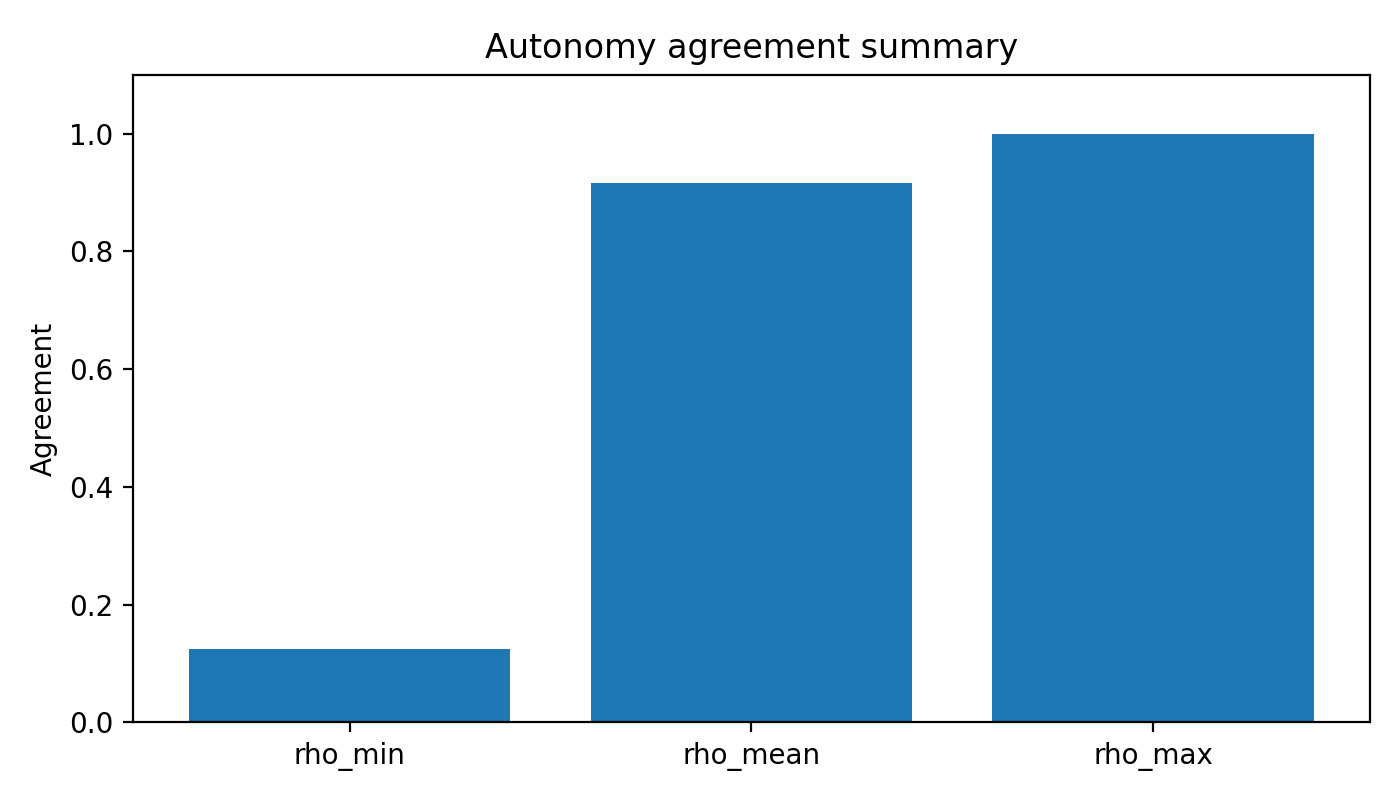
\includegraphics[width=0.9\columnwidth]{../results/figures/fig_autonomy_agreement.png}
\caption{Agreement summary from the autonomy-layer export. The run remained non-convergent (\texttt{converged = False}) after \texttt{200} rounds despite high mean agreement.}
\label{fig:autonomy_agreement}
\end{figure}


\subsection{Compression and Fidelity}

The exported compression table reported a compression ratio of \texttt{9.23076923076923} and provided full-versus-compressed values for the metrics listed below.


\noindent\textbf{Table 3.} Full-network versus compressed-network fidelity summary.

\begin{table}[t]
\centering
\caption{Full-network versus compressed-network fidelity summary.}
\label{tab:compression_fidelity}
\small
\begin{tabular}{lcc}
\hline
Metric & Full network & Compressed network \\
\hline
global\_efficiency & 0.0976056277 & 0.2846139149 \\
avg\_path\_length & inf & inf \\
modularity & 0.9022723828 & N/A \\
lcc\_fraction & 0.9753333333 & N/A \\
compression\_ratio & 9.2307692308 & N/A \\
\hline
\end{tabular}
\end{table}

The exported fidelity table reported different \texttt{global\_efficiency} values for the full and compressed representations and reported \texttt{avg\_path\_length = inf} for both. Compressed-network entries for \texttt{modularity}, \texttt{lcc\_fraction}, and \texttt{compression\_ratio} were not populated in the current CSV export. This means that compression may still be useful as a tractability device for larger constellation or observation-network studies, but the present evidence does not justify assuming that every structural property relevant to coordination-sensitive observation tasks is preserved after coarsening.

\begin{figure}[t]
\centering
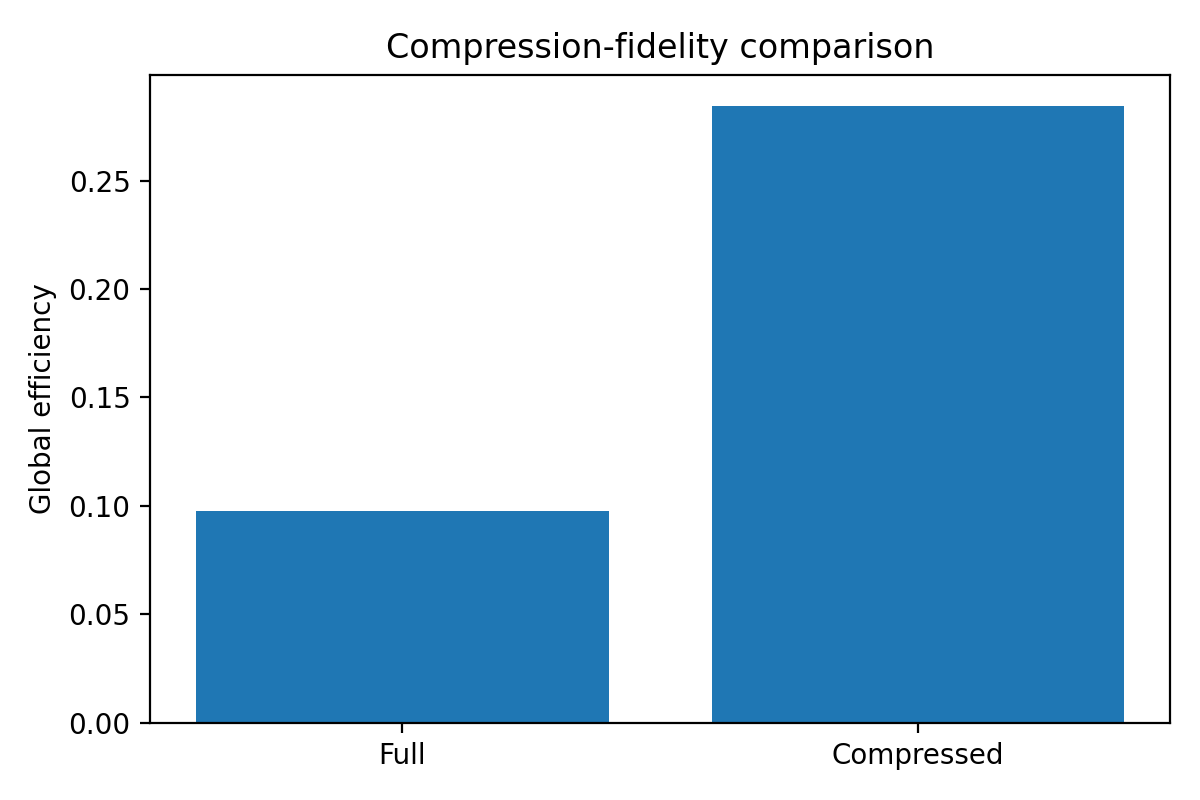
\includegraphics[width=0.78\columnwidth]{../results/figures/fig_compression_efficiency.png}
\caption{Compression-fidelity comparison on the finite metric exported for both representations. \texttt{avg\_path\_length} remained \texttt{inf} in both cases, while other compressed-network entries were not exported.}
\label{fig:compression_efficiency}
\end{figure}


\section{DISCUSSION}

The central question of this study was whether a reproducible enhanced pipeline could preserve the structural outputs of the regular pipeline while also producing an interpretable autonomy-layer outcome on the same satellite-derived graph. The present evaluation answered that question in a narrow but useful way. Structural parity held across the reported full-network metrics, but the autonomy layer did not converge within the declared horizon. Taken together, these findings supported a calibration interpretation: the downstream structural measurement stack appeared stable under the enhanced insertion, whereas the decision dynamics remained unresolved under the current configuration.


\subsection{Principal Interpretation}

The structural parity result mattered because it reduced one important source of ambiguity. Since the regular and enhanced branches produced identical reported structural metrics on the same graph instance, the autonomy insertion did not introduce visible drift into the exported Stage 2 and Stage 3 outputs. This narrowed the interpretation space for the study: the unresolved autonomy outcome was not, on the present evidence, best explained as a hidden change in graph construction or structural measurement. Instead, it pointed attention toward the dynamics of the autonomy layer itself and to the declared convergence rule used to evaluate it.

The autonomy result required equally careful framing. High mean local agreement together with no global decision under a bounded horizon did not justify either a success claim or a blanket failure claim. It showed that, for this graph and this parameterization, local coordination signals were not sufficient to satisfy the full convergence test within the allowed rounds. Neighbor-interaction theory has long emphasized that convergence depends on topology, update rules, and switching behavior rather than following automatically from local connectivity alone.[4,6,7] In that sense, the present result fit established theory better than it contradicted it.

For the paper's planetary-observation framing, the interpretation is enabling rather than direct. Future distributed observation architectures may eventually use coordination logic to decide how multiple assets prioritize targets, share sensing opportunities, or respond to changing conditions. Under that broader application view, a bounded-horizon non-convergence result matters because unresolved collective state could map, in principle, to delayed retargeting, ambiguous observation priorities, or missed sensing opportunities. The present paper does not model those mission outcomes directly, but it does identify a prerequisite that would have to be calibrated before such observation concepts could be treated more confidently.


\subsection{Context Within Existing Literature}

The result also aligned with broader work on decentralized collective decisions. Studies of spacecraft swarms and distributed control have shown that local coordination, thresholding, and information aggregation can produce regimes in which partial agreement does not yield a single certified global resolution on the time scale imposed by the control law or planning horizon.[2,3,7] The current evaluation extended that general lesson into the paper's specific setting: a notional satellite-derived kNN graph with a declared convergence rule and a fixed autonomy horizon.

At the same time, the study did not claim equivalence between the present graph abstraction and operational spacecraft communications. The edges remained declared modeling constructs rather than measured links, and the autonomy outcome therefore remained evidence about a computational model under stated assumptions. That limitation did not nullify the result; it defined the level at which the result should be believed. The contribution was thus methodological and calibrative: a reproducible record that separated structural invariance from decision-dynamical resolution.

This distinction is also what connects the study to autonomous observation literature without overstating its scope. Work in remote sensing, adaptive observation, and machine-assisted geoscience increasingly argues that future scientific return will depend on systems that can manage dynamic targets, onboard resource limits, and distributed measurement opportunities.[9,11,12,15,16,17,18] The present paper does not solve those mission-level problems. It instead evaluates whether one candidate coordination substrate behaves in a reproducible and interpretable way, which is a narrower but necessary step toward any future observation architecture that would rely on autonomous multi-satellite decision processes.

The compression result should be read in the same disciplined way. The compressed representation preserved neither every reported metric nor strict equality with the full graph, and it was not expected to do so. Graph coarsening is generally an approximation that trades representational fidelity for tractability, so the relevant question was not whether the compressed graph was identical to the original one, but whether the observed departures were acceptable for the intended use.[6] In the present manuscript, that question remained open for autonomy-oriented uses and should not be answered more strongly than the current evidence allowed. For future observation-oriented studies, the same caution would apply to any use of compressed representations for scheduling, retargeting, or distributed sensing logic.


\subsection{Limitations and Calibration Agenda}

Several limitations constrained the transferability of these conclusions. First, the study evaluated one frozen graph-construction rule and one logged autonomy configuration rather than a broad parameter sweep. Second, the graph was a notional interaction scaffold derived from orbital-element features rather than a validated communications network. Third, the current artifact set still required completion of several provenance and environment details before the reproducibility package could be considered fully submission-ready. Fourth, the reported run was bounded by a fixed stopping horizon, so the result distinguished only between convergence within that horizon and non-convergence within that horizon.

These limitations clarified, rather than weakened, the next research moves. The most immediate calibration agenda was to vary stopping horizon, agreement and variance thresholds, edge-weight construction, initialization choices, and graph-construction assumptions while preserving the same artifact discipline. A second priority was to determine which quantities must remain invariant for the compressed representation to be considered adequate for autonomy studies rather than for structural summaries alone. A third priority was to complete the provenance and environment record so that third-party reproductions could test whether the same negative result reproduced under identical conditions. A fourth priority, if the framework is to be connected more directly to planetary observation, would be to define mission-relevant proxy tasks such as bounded retargeting, opportunity allocation, or observation scheduling and then test whether the calibrated coordination layer improves or constrains those tasks under controlled assumptions.

The most defensible high-level conclusion from this section was therefore narrow: structural stability of the reported pipeline did not imply bounded-horizon decision resolution in the autonomy layer. That statement answered the study objective directly, remained consistent with the cited consensus and collective-decision literature, and avoided upgrading a calibration finding into an operational autonomy claim.

No additional discussion figure was included. The calibration roadmap is summarized in prose as: structural parity established $\rightarrow$ bounded-horizon non-convergence observed $\rightarrow$ future sensitivity analysis over horizon, thresholds, edge-weight construction, initialization, and graph assumptions.


\section{INDUSTRY IMPLICATIONS}

The operational implication of this evaluation was narrow and practical. The reported structural parity showed that the enhanced insertion did not disturb the downstream structural measurement stack, but the autonomy layer did not converge within the declared horizon. For industry readers, that combination supported a gating posture rather than an autonomy-readiness claim. In the specific context of planetary and remote-observation programs, the relevant near-term use case is not unsupervised mission authority, but bounded support for adaptive targeting, distributed observation scheduling, and other advisory coordination functions.

For mission operators and autonomy integrators, the present evidence supported using this class of autonomy layer only in advisory, shadow-mode, or offline analysis roles until convergence had been demonstrated under declared horizons and controlled evaluations. That recommendation was consistent with current small-satellite autonomy practice rather than unusually conservative: flight demonstrations and autonomous navigation studies have generally been introduced as bounded technology-development steps rather than as blanket authorization for fully autonomous control.[1,13,14] In the same spirit, the current evaluation supported a staged deployment logic for observation programs as well: first calibration, then monitored advisory use for target selection or scheduling, and only later any consideration of higher autonomy authority if convergence evidence improves.

For smallsat and remote-observation programs specifically, the paper's recommendation aligned with real platform constraints. Small satellites expose autonomy weaknesses quickly because compute, communications windows, and operational margins are tighter than in larger mission classes. At the same time, observation missions increasingly seek better temporal coverage, rapid response to transient phenomena, and more efficient use of onboard resources, all of which increase pressure for adaptive onboard coordination.[11,12,16,17,18] Spacecraft-swarm demonstrations, autonomous navigation research, and automated science-planning systems all point toward the same operational lesson: onboard autonomy is most credible when introduced first as bounded task allocation, decision support, or planning assistance under explicit constraints.[1,5,10,13,14]

For program managers and system architects, the most actionable implication was where not to spend effort. The parity result suggested that immediate redesign of the structural pipeline was not the first priority. The higher-value next investment was sensitivity testing of the autonomy layer itself, including horizon length, convergence thresholds, initialization choices, and edge-weight construction, because that was where the unresolved behavior remained visible in the current evidence base. For observation architectures, this means that claims about autonomous retargeting, opportunistic sensing, or coordinated measurement scheduling should remain provisional until the underlying coordination dynamics are shown to resolve under mission-relevant bounds. This recommendation also matched the broader distributed-spacecraft literature, which repeatedly treats graph topology, weighting, and timing assumptions as primary determinants of convergence behavior rather than secondary implementation details.[2,3,4,6,7]

For assurance and governance stakeholders, the study reinforced the need for explicit decision gates before any autonomy feature is allowed to influence mission-level coordination. At minimum, such gates should require reproducible evaluations on the same artifact package, documented convergence criteria, and evidence that non-convergence modes are detectable and operationally containable. Constellation-management and automated science-planning practice already point in this direction: operational autonomy advances through bounded workflows, constraint checks, and monitored oversight rather than reliance on agreement statistics alone.[5,10]

The most defensible industry recommendation from this paper was therefore specific: \textbf{do not automate global coordination decisions from this autonomy layer until convergence is reproduced under declared horizons, stress-tested across controlled evaluations, and tied to explicit operational safety gates}. Under the current evidence, the autonomy layer was best treated as a calibration instrument that could inform engineering judgment without yet carrying independent decision authority. For planetary-observation and remote-sensing programs, that means the near-term value lies in advisory support for bounded targeting or scheduling experiments rather than autonomous control of mission-level observation decisions. Short term, that meant advisory and shadow-mode use; medium term, it meant bounded-horizon sensitivity studies tied to mission-relevant failure cases; long term, it meant considering greater authority only after reproducible convergence and assurance evidence had been established.

No additional industry-facing figure was included. The staged adoption logic is summarized in prose as: calibration $\rightarrow$ advisory or shadow-mode use $\rightarrow$ gated operational use only after reproducible convergence evidence and assurance review.


\section{CONCLUSIONS}

This study answered its central question in a deliberately narrow way. The reported evaluation showed that the enhanced pipeline preserved the structural outputs of the regular pipeline on the same graph instance, but it did not produce bounded-horizon convergence in the autonomy layer under the declared configuration. The main contribution of the paper is therefore methodological rather than triumphalist: it establishes a reproducible calibration record showing that structural stability and decision-dynamical resolution are separable outcomes in this notional satellite-graph setting.

That conclusion matters because it gives the field a cleaner next step. Planetary observation increasingly depends on distributed and adaptive architectures, but those architectures require coordination layers that can be audited before they can be trusted. The appropriate response to the present result is therefore neither to claim operational autonomous observation nor to discard the framework, but to use the same artifact-governed workflow to map convergence regimes more carefully. Future calibration studies should vary stopping horizons, threshold rules, graph-construction assumptions, initialization choices, and autonomy-update settings while preserving the reproducibility discipline established here, and then connect those calibrated dynamics to controlled observation-oriented proxy tasks such as retargeting or scheduling. If those follow-on studies succeed, this framework may mature into a stronger basis for autonomy assessment in future planetary-observation architectures; if they continue to expose non-convergent regimes, that outcome will remain scientifically valuable because it defines the operating boundaries of the model rather than hiding them.


\section*{ACKNOWLEDGMENTS}

The author gratefully acknowledges Nebula Research Lab Advisors, Shelli Brunswick for her valuable contributions and thoughtful guidance while advising Nebula Research Lab towards the venture capital sector. The author also thanks Gennady Shenker for his sustained guidance and deep commercial knowledge, which helped advance this line of research into an academic context. In addition, the author acknowledges Robi Sen for his insightful perspective on defense-industry considerations relevant to the broader framing of this work. The collective support and expertise of these individuals helped shape the development of the research presented in this paper.

\section{REFERENCES}
\begin{enumerate}
\item Kruger, J., Hwang, S., and D'Amico, S., "Starling Formation-Flying Optical Experiment: Initial Operations and Flight Results," \emph{Proceedings of the 38th Annual AIAA/USU Conference on Small Satellites}, Logan, UT, 2024.
\item Morgan, D., Chung, S.-J., and Hadaegh, F. Y., "Model predictive control of swarms of spacecraft using sequential convex programming," \emph{Journal of Guidance, Control, and Dynamics}, Vol. 37, No. 6, pp. 1725-1740, 2014.
\item Ramirez-Riberos, J. L., Pavone, M., Frazzoli, E., and Miller, D. W., "Distributed control of spacecraft formations via cyclic pursuit: Theory and experiments," \emph{Journal of Guidance, Control, and Dynamics}, Vol. 33, No. 5, pp. 1655-1669, 2010.
\item Jadbabaie, A., Lin, J., and Morse, A. S., "Coordination of groups of mobile autonomous agents using nearest neighbor rules," \emph{IEEE Transactions on Automatic Control}, Vol. 48, No. 6, pp. 988-1001, 2003.
\item Choo, T. H., Berman, A. F., Nair, H., Nguyen, L., Skura, J. P., and Steele, R. J., "SciBox: An autonomous constellation management system," \emph{Johns Hopkins APL Technical Digest}, Vol. 33, No. 4, 2017.
\item Mesbahi, M., and Egerstedt, M., \emph{Graph Theoretic Methods in Multiagent Networks}, Princeton University Press, Princeton, NJ, 2010.
\item Olfati-Saber, R., "Flocking for multi-agent dynamic systems: Algorithms and theory," \emph{IEEE Transactions on Automatic Control}, Vol. 51, No. 3, pp. 401-420, 2006.
\item CelesTrak, "Current GP Element Sets," \url{https://celestrak.org/NORAD/elements/}. Constellation-specific JSON endpoints used in this study were \texttt{gp.php?GROUP=iridium-NEXT\&FORMAT=json}, \texttt{gp.php?GROUP=oneweb\&FORMAT=json}, and \texttt{gp.php?GROUP=starlink\&FORMAT=json}. Exact local retrieval UTC for the archived JSON files was not preserved in the current artifact bundle.
\item Nebula Research Lab Commits, "NRL-M5-SatSim: Satellite Autonomy for Planetary Ecological Observation," GitHub repository, \url{https://github.com/nebularesearchlab-commits/NRL-M5-SatSim}.
\item Francis, R., Estlin, T., Doran, G., Johnstone, S., Gaines, D., Verma, V., Burl, M., Frydenvang, J., Montano, S., Wiens, R. C., Schaffer, S., Gasnault, O., DeFlores, L., Blaney, D., and Bornstein, B., "AEGIS autonomous targeting for ChemCam on Mars Science Laboratory: Deployment and results of initial science team use," \emph{Science Robotics}, Vol. 2, No. 7, eaan4582, 2017. doi:10.1126/scirobotics.aan4582.
\item Choo, T. H., Murchie, S. L., Bedini, P. D., Steele, R. J., Skura, J. P., Nguyen, L., Nair, H., Lucks, M., Berman, A. F., McGovern, J. A., and Turner, F. S., "SciBox, an end-to-end automated science planning and commanding system," \emph{Acta Astronautica}, Vol. 93, pp. 490-508, 2014.
\item Dubovik, O., Schuster, G. L., Xu, F., Hu, Y., Bosch, H., Landgraf, J., and Li, Z., "Grand Challenges in Satellite Remote Sensing," \emph{Frontiers in Remote Sensing}, Vol. 2, 619818, 2021. doi:10.3389/frsen.2021.619818.
\item Knobelspiesse, K., and Nag, S., "Remote sensing of aerosols with small satellites in formation flight," \emph{Atmospheric Measurement Techniques}, Vol. 11, pp. 3935-3954, 2018. doi:10.5194/amt-11-3935-2018.
\item Kruger, J. J., \emph{Flight Algorithms for Autonomous Tracking and Navigation of Distributed Space Systems Using Inter-Satellite Bearing Angles}, Ph.D. Dissertation, Stanford University, Stanford, CA, 2024.
\item Sullivan, J. A., \emph{Nonlinear Angles-Only Orbit Estimation for Autonomous Distributed Space Systems}, Ph.D. Dissertation, Stanford University, Stanford, CA, 2020.
\item Chakraborty, S., \emph{Advanced Processing of Multispectral Satellite Data for Detecting and Learning Knowledge-based Features of Planetary Surface Anomalies}, Ph.D. Dissertation, Arizona State University, Tempe, AZ, 2022.
\item Chien, S., Zilberstein, I., Candela, A., Rijlaarsdam, D., Hendrix, T., Dunne, A., Oriol, A., and Puig, M. J., "Flight of Dynamic Targeting on the CogniSAT-6 Spacecraft," \emph{Proceedings of the International Symposium on Artificial Intelligence, Robotics and Automation in Space (i-SAIRAS)}, 2024. arXiv:2509.05304.
\item Reichstein, M., Camps-Valls, G., Stevens, B., Jung, M., Denzler, J., Carvalhais, N., et al., "Deep learning and process understanding for data-driven Earth system science," \emph{Nature}, Vol. 566, No. 7743, pp. 195-204, 2019. doi:10.1038/s41586-019-0912-1.
\item Lary, D. J., Alavi, A. H., Gandomi, A. H., and Walker, A. L., "Machine learning in geosciences and remote sensing," \emph{Geoscience Frontiers}, Vol. 7, No. 1, pp. 3-10, 2016. doi:10.1016/j.gsf.2015.07.003.
\end{enumerate}

\end{multicols}

\end{document}
